\documentclass[default]{beamer}
\setbeamertemplate{navigation symbols}{}

\usetheme{CambridgeUS}
\useoutertheme{infolines}
%\usecolortheme{crane}

\usepackage{cmap}							% Поддержка поиска русских слов в PDF (pdflatex)
\usepackage[T2A]{fontenc}       			%поддержка кириллицы
\usepackage[utf8]{inputenc}					% Выбор языка и кодировки
\usepackage[english, russian]{babel}
\usepackage{csquotes}
\usepackage{tikz}
\usetikzlibrary{calc}

\usepackage[
	language=auto,
	autolang=other,
	backend=biber,
	style=authortitle,
	sorting=ydnt
]{biblatex}
\addbibresource{tononi.bib}
				
\DeclareSourcemap{
	\maps[datatype=bibtex, overwrite]{
		\map{
			\step[fieldset=langid, fieldvalue=english]
			\step[fieldset=doi, null]
			\step[fieldset=issn, null]
			\step[fieldset=isbn, null]
			\step[fieldset=url, null]
			\step[fieldsource=language, fieldset=langid, origfieldval]
		}
	}
}


\graphicspath{{../../images/}} 			% Пути к изображениям

\makeatletter
\setbeamertemplate{footline}
{
	\leavevmode%
	\hbox{%
		\begin{beamercolorbox}[wd=.333333\paperwidth,ht=2.25ex,dp=1ex,center]{author
				in head/foot}%
			\usebeamerfont{author in
				head/foot}\insertshortauthor~~\beamer@ifempty{\insertshortinstitute}{}{(\insertshortinstitute)}
		\end{beamercolorbox}%
		\begin{beamercolorbox}[wd=.333333\paperwidth,ht=2.25ex,dp=1ex,center]{title in
				head/foot}%
			\usebeamerfont{title in head/foot}\insertshorttitle
		\end{beamercolorbox}%
		\begin{beamercolorbox}[wd=.333333\paperwidth,ht=2.25ex,dp=1ex,right]{date in
				head/foot}%
			\usebeamerfont{date in head/foot}\insertshortdate{}\hspace*{2em}
			\insertframenumber{}\hspace*{2ex} 
		\end{beamercolorbox}
	}%
	\vskip0pt%
}


\renewcommand*{\bibfont}{\footnotesize}

\begin{document}
	
	\title[Bio- and psycho-inspired methods in AI]{Биологически и психологически правдоподобные методы моделирования в искусственном интеллекте}
	\author[Панов]{Александр Панов}
	\institute[ФИЦ ИУ РАН]{Федеральный исследовательский центр <<Информатика и управление>> РАН}
	\date{18 марта 2016~г.} 
	
	\begin{frame}
		\titlepage
	\end{frame}
	
	\begin{frame}
		\frametitle{Новая парадигма исследований в ИИ}
		
		\begin{itemize}
			\item Искусственный интеллект исследует средства решения интеллектуальных задач, т.е. таких задач, которые не имеют известного алгоритма решения.
			\item Компьютерная аналогия перестала отвечать новым требованиям, предъявляемых к интеллектуальным задачам.
			\item Необходимо рассмотреть науку <<Искусственный интеллект>> в контексте всех когнитивных наук.
			\item В этом случае целью искусственного интеллекта становится построение правдоподобных гипотез (моделей) работы когнитивных функций человека, которые бы согласовывались как с экспериментальными данными когнитивных психологов, так и с нейрофизиологическими данными о строении и функционировании мозга человека.
		\end{itemize}
	\end{frame}

	\begin{frame}
		\frametitle{Биологическое и психологическое правдоподобие}
		
		Возникает потребность в разработке новых биологически и психологически правдоподобных методов(biologically and psychologically inspired methods)  моделирования когнитивных функций в искусственном интеллекте.
		\par\bigskip
		Пример:
		\begin{itemize}
			\item использование\textit{ культурно-исторического подхода} и  \textit{психологической теории деятельности} (Лурия, Выготский, Леонтьев), как основы описания работы когнитивных функций,
			\item использование идей\textit{ прикладной семиотики} (Поспелов, Осипов),
			\item использование моделей работы\textit{ кортикальной колонки} (Маунткасл, Хокинс) и \textit{нейронного ансамбля} (Эйдельман, Инваницкий) в качестве нейрофизиологического <<заземления>> (grounding).
		\end{itemize}
	\end{frame}

	\begin{frame}
		\frametitle{Знаковая картина мира}
		
		\begin{columns}
			\begin{column}{0.6\textwidth}
				\begin{itemize}
					\item Модель представления субъекта о действительности "--- картина мира.
					\item Элемент картины мира "--- знак, четырх-компонентная структура.
					\item Знаки опосредуют как объекты, так и процессы, ситуации, внутренние характеристики и т.п.
				\end{itemize}
			\end{column}
			\begin{column}{0.4\textwidth}
				\begin{figure}
					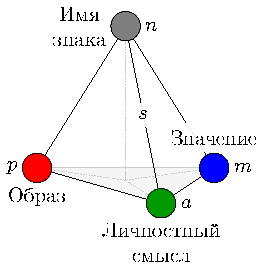
\includegraphics[width=0.7\textwidth]{signs/sign_colored}
				\end{figure}

				\begin{tikzpicture}[scale=1, every node/.style={scale=0.85}]

				\node[align=center] at (0,0) {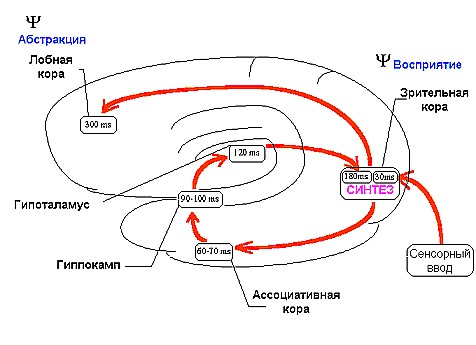
\includegraphics[width=1.1\textwidth]{phisio/ivanitsky_cyrcle}};
				
				\node (tmp1) at (2.7,-2) {};
				\node (tmp2) at (2.9,-0.8) {};
				\node (tmp3) at (3.9,0) {};
				\node (tmp4) at (4.9,0.6) {};
				
				\node (tmp5) at (5,0.75) {};
				\node (tmp6) at (6,0.15) {};
				
				\draw[thick, blue] (0.9,-0.1) circle (0.3);
				\draw[thick, blue] (-0.4,-0.3) circle (0.3);
				\draw[thick, blue] (0,0.2) circle (0.3);
				\end{tikzpicture}
			\end{column}
		\end{columns}
	\end{frame}

	\begin{frame}
		\frametitle{Уровни представления}
		
		\begin{figure}
			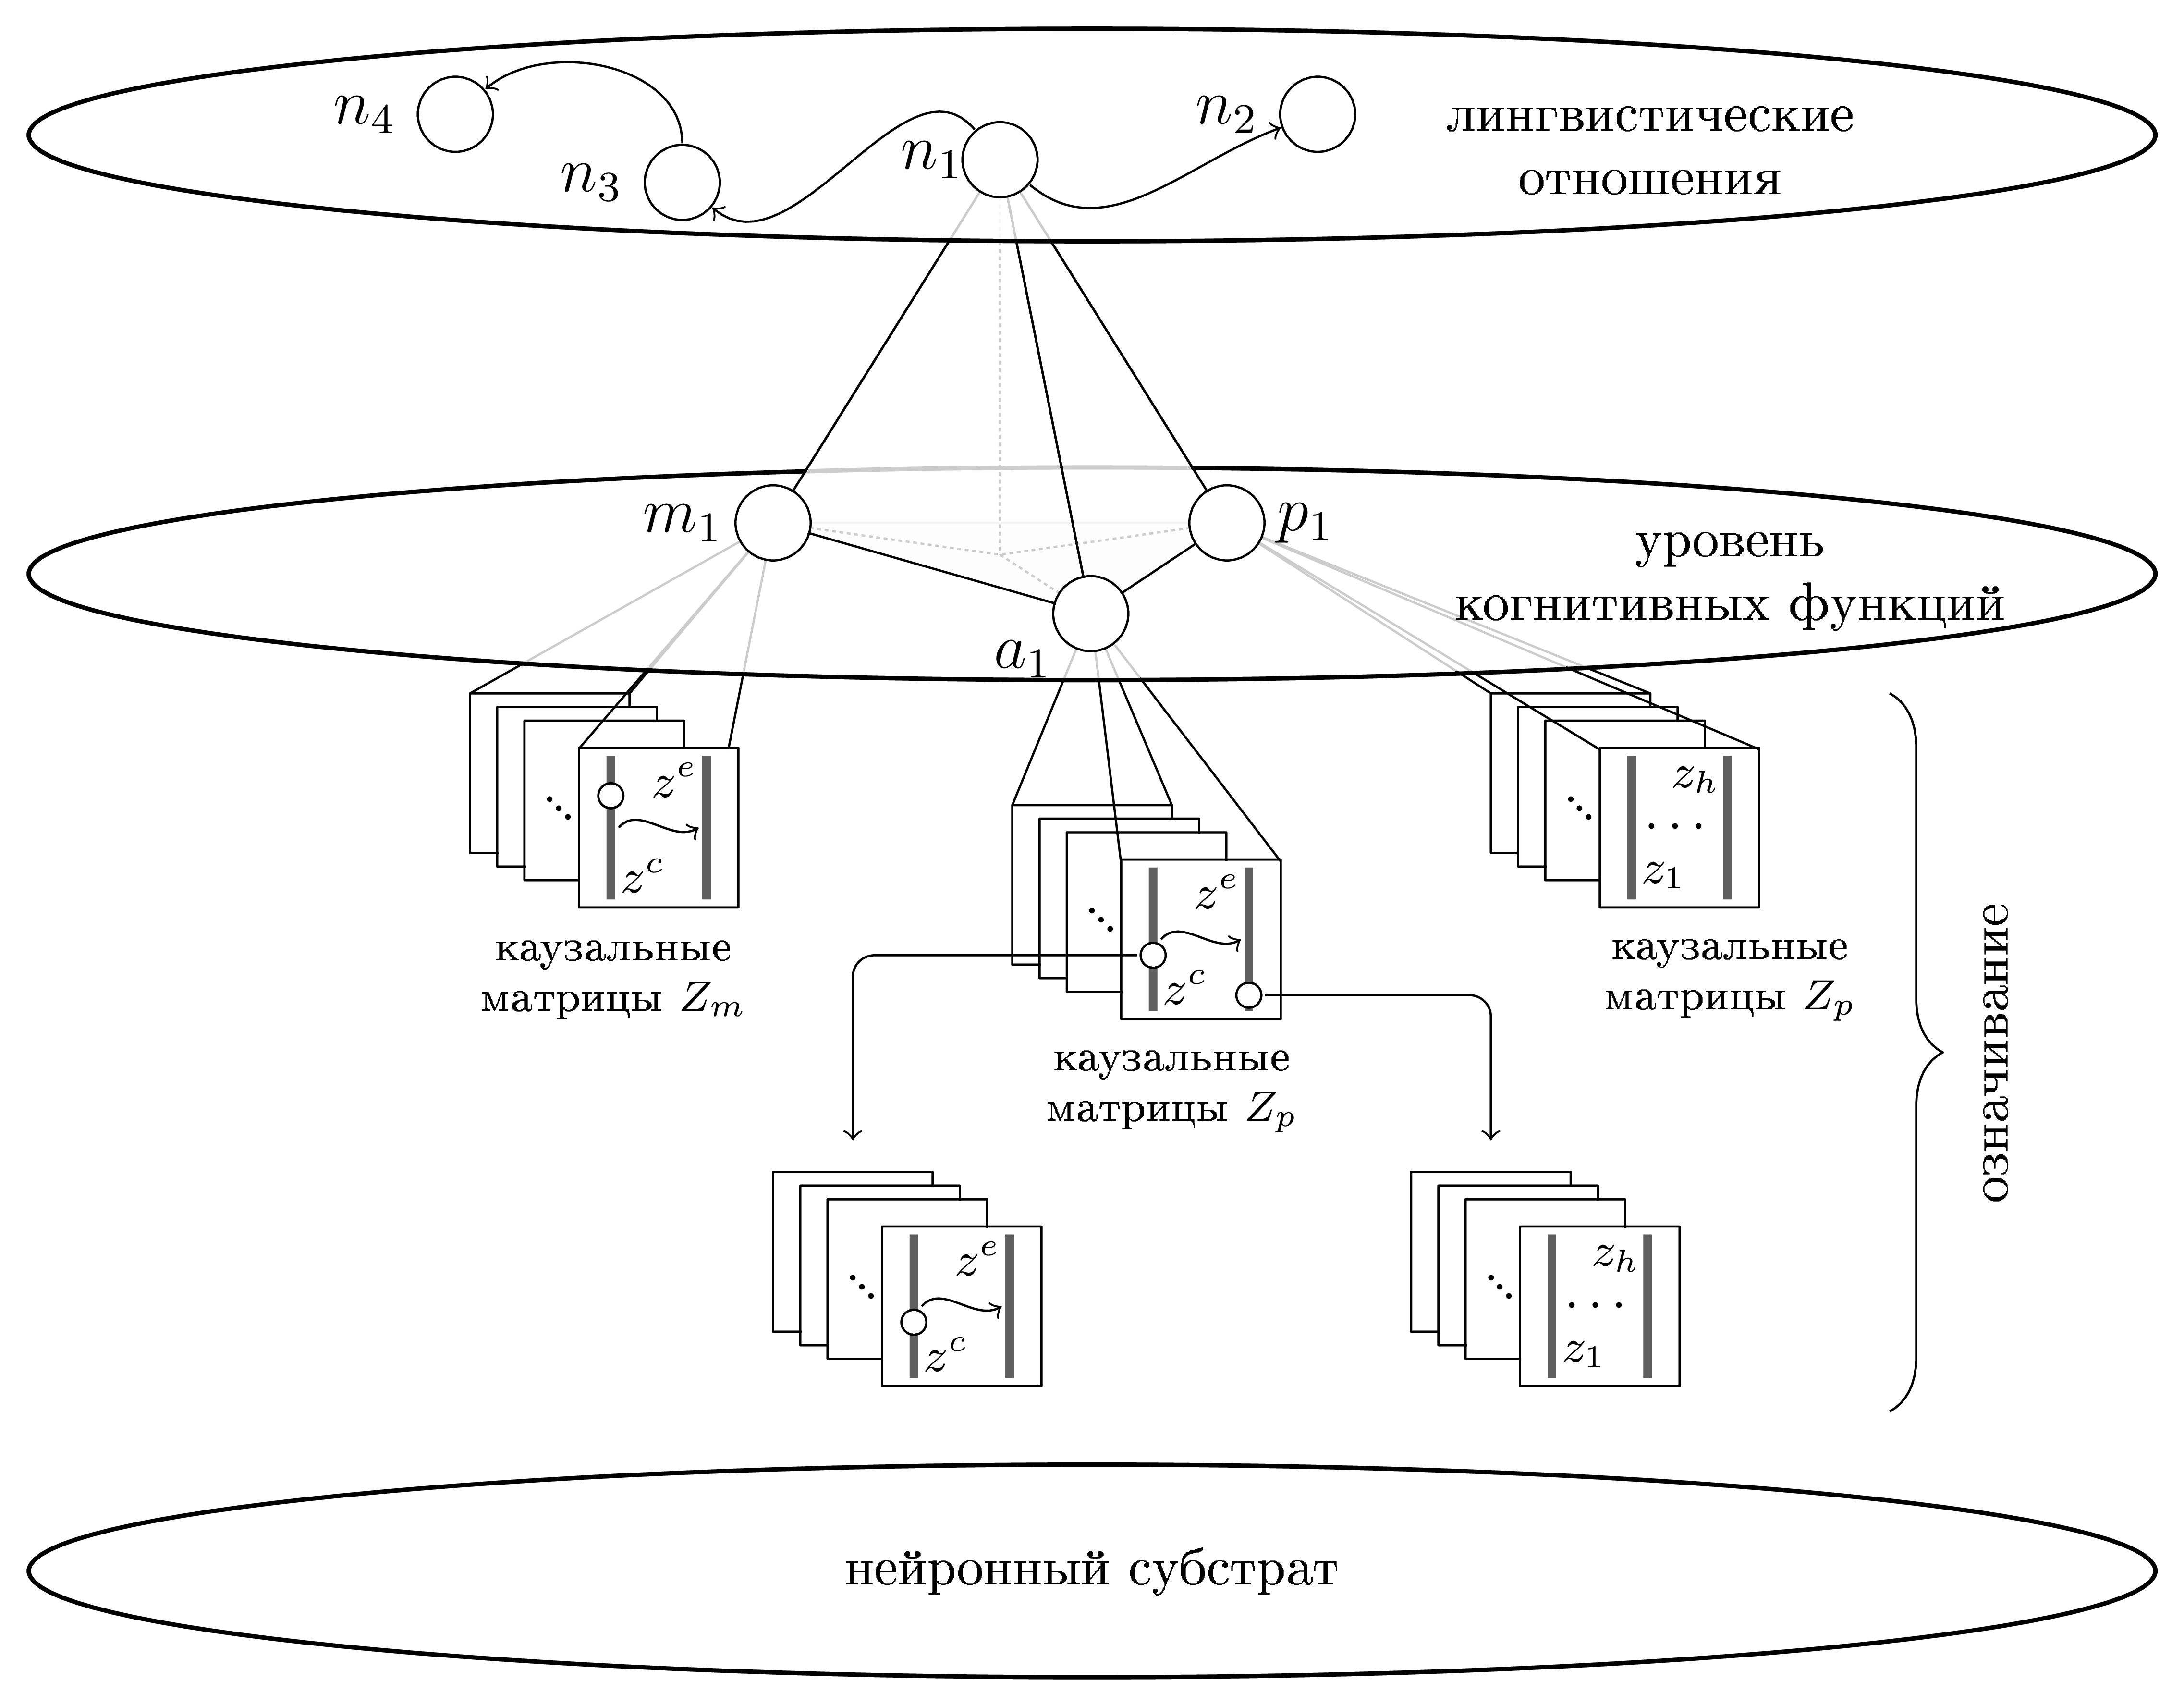
\includegraphics[width=0.7\textwidth]{signs/sign_levels}
		\end{figure}
	\end{frame}

	\begin{frame}
		\frametitle{Знаковая модель}
		
		\begin{itemize}
			\item Когнитивные функции "--- это процессы, качественно зависимые от субстрата и воспроизводимые с помощью вычислений (<<заземленная>> структура компонент знака).
			\item Вместо когнитивного солипсизма "--- взаимодействие с внешней средой (теория деятельности, сигналы внешней среды).
			\item Системный подход в задании причинно-следственных связей (пространство состояний по Тонони).
			\item Необходимость коллективного взаимодействия в процессе обучения и действования.
		\end{itemize}
	\end{frame}

	\begin{frame}
		\frametitle{Картина мира субъекта деятельности}
		
		\begin{columns}
			\begin{column}{0.55\textwidth}
				\begin{figure}
					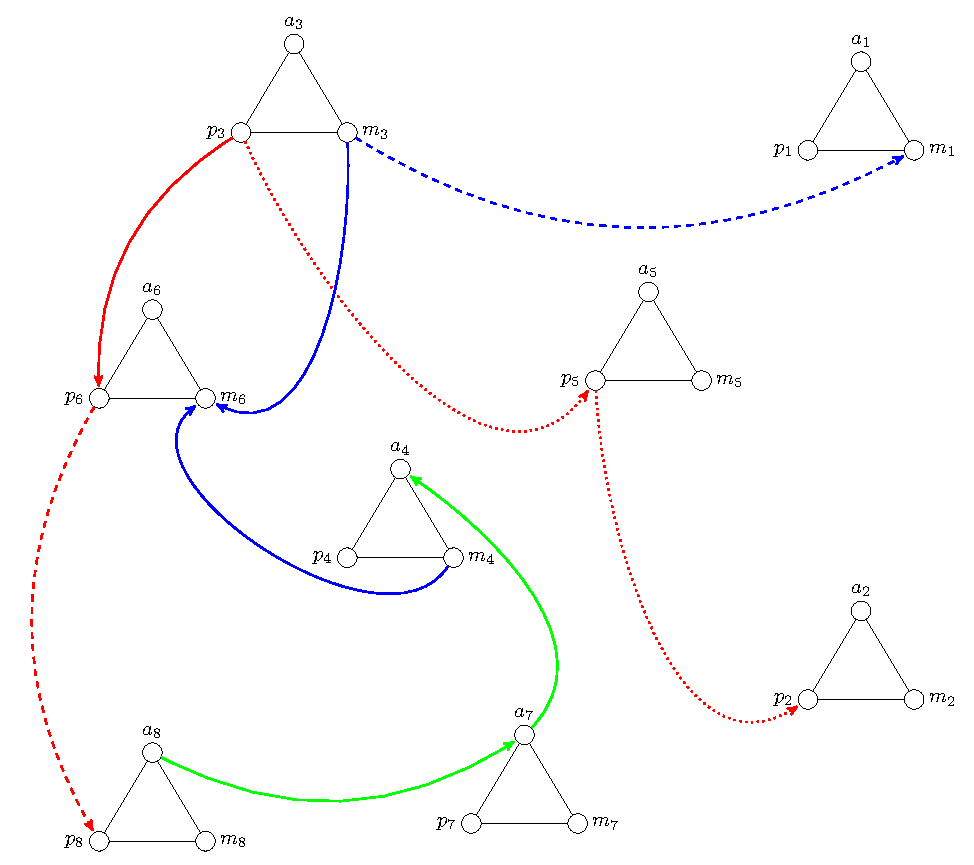
\includegraphics[width=\textwidth]{signs/signs_net}
				\end{figure}
			\end{column}
			\begin{column}{0.45\textwidth}
				\textit{Семиотическая сеть} $H=\langle H_P, H_A, H_M\rangle$, где
				\begin{itemize}
					\item $H_P=\langle2^P,\mathfrak R_P\rangle$ "--- семантическая сеть на множестве образов знаков,
					\item $H_P=\langle2^A,\mathfrak R_A\rangle$ "--- семантическая сеть на множестве значений знаков,
					\item $H_P=\langle2^M,\mathfrak R_M\rangle$ "--- семантическая сеть на множестве личностных смыслов знаков.
				\end{itemize}
			\end{column}
		\end{columns}
	\end{frame}		

	\begin{frame}
		\frametitle{Нейронный субстрат}
		
		\begin{columns}
			\begin{column}{0.5\textwidth}
				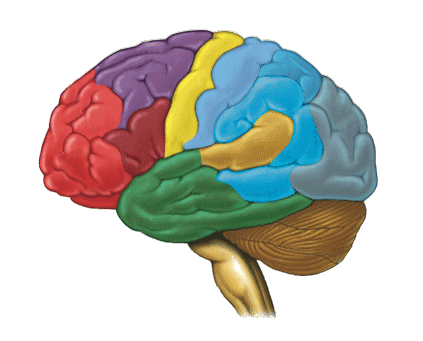
\includegraphics[width=0.7\textwidth]{phisio/mozg_2}
				\par\bigskip
				\hspace{-7mm}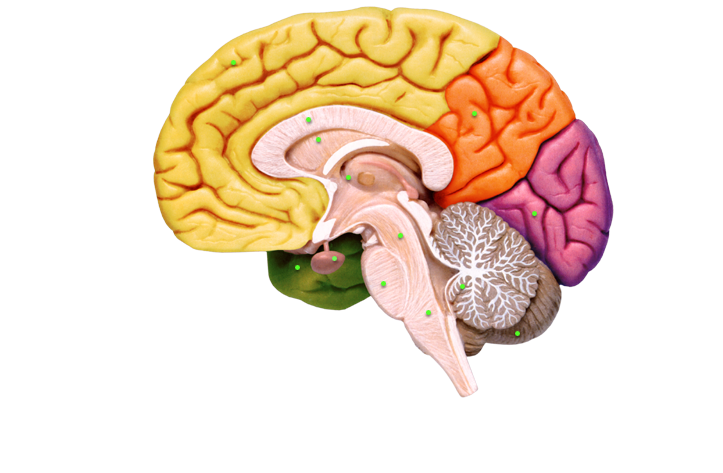
\includegraphics[width=0.9\textwidth]{phisio/mozg}
			\end{column}
			\begin{column}{0.5\textwidth}
				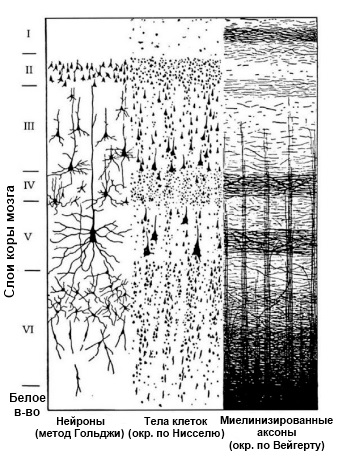
\includegraphics[width=0.9\textwidth]{phisio/column_layers_ru}
			\end{column}
		\end{columns}
	\end{frame}
	
	\begin{frame}
		\frametitle{Основные свойства модели и используемые упрощения}
		
		\begin{columns}
			\begin{column}{0.3\textwidth}
				\begin{figure}
					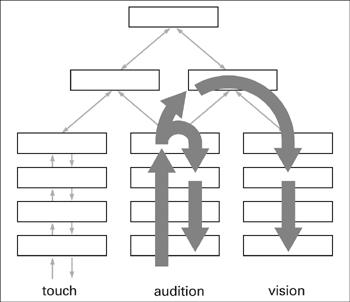
\includegraphics[width=\textwidth]{mpf/info_flow.jpg}
				\end{figure}
			\end{column}
			\begin{column}{0.7\textwidth}
				\begin{overlayarea}{\textwidth}{0.7\textheight}
					\only<1>{
						Принимается следующие гипотезы:
						\begin{itemize}
							\item неокортекс состоит из зон (регионов), состоящих в свою очередь из колонок и имеющих одинаковое строение на всех участках коры;
							\item колонки в регионе объединены латеральными связями;
							\item таламус формирует последовательности паттернов за счет задержки возбуждения/торможения.
						\end{itemize}
					}
					
					\only<2>{
						Основные свойства:
						\begin{itemize}
							\item хранение последовательности паттернов в инвариантной форме,
							\item воспроизведение паттернов автоассоциативно,
							\item хранение паттернов в иерархической системе,
							\item использование обратной связи для предсказания поступающей на данный уровень иерархии информации. 
						\end{itemize}
					}
					
					\only<3>{
						Упрощения:
						\begin{itemize}
							\item дискретность во времени,
							\item простейшая строгая иерархия со связями только между
							ближайшими уровнями,
							\item гипотеза одинаковой длительности распознаваемых явлений в рамках одного региона,
							\item пороговая модель принятия решений в случае неопределенности результата распознавания,
							\item подавление непредвиденного сигнала,
							\item отсутствие моторной составляющей обратной связи.
						\end{itemize}
					}				
				\end{overlayarea}
			\end{column}
		\end{columns}
	\end{frame}
	
	\begin{frame}
		\frametitle{Формальная модель нейрона}
		
		\begin{center}
			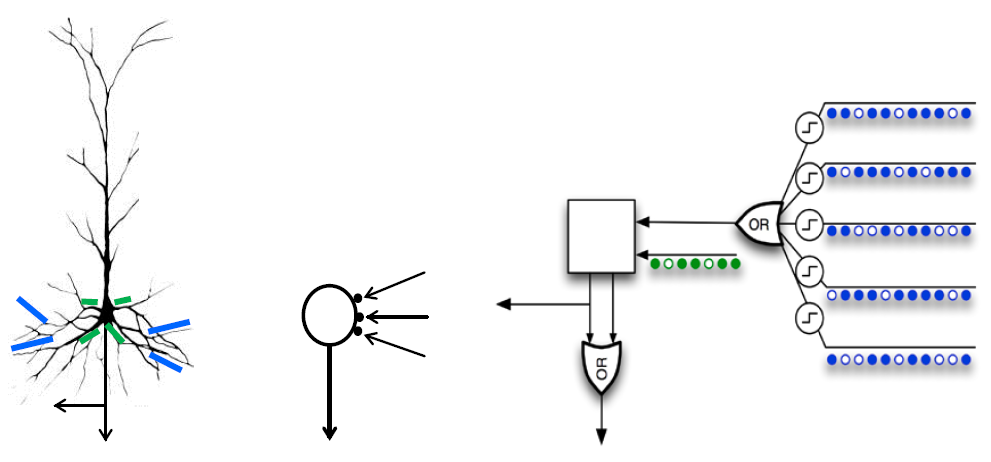
\includegraphics[width=0.9\textwidth]{phisio/neuro_htm}
		\end{center}
		
		\begin{itemize}
			\item Проксимальный дендритный сегмент "--- прямая активация.
			\item Дистальные дендритные сегменты "--- латеральный вход и состояние предсказания.
		\end{itemize}
	\end{frame}
	
	\begin{frame}
		\frametitle{Иерархическая организация нейронов}
		
		\begin{columns}
			\begin{column}{0.5\textwidth}
				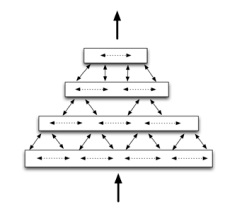
\includegraphics[width=0.9\textwidth]{mpf/hierarchy}
			\end{column}
			\begin{column}{0.5\textwidth}
				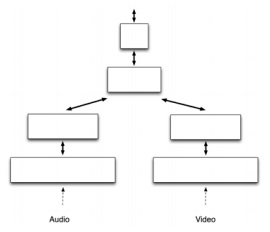
\includegraphics[width=0.9\textwidth]{mpf/hierarchy_conv}
			\end{column}
		\end{columns}
		
	\end{frame}
	
	\begin{frame}
		\frametitle{Иерархическая модель}
		
		
		\begin{overlayarea}{\textwidth}{\textheight}
			\only<1>{
				\begin{center}
					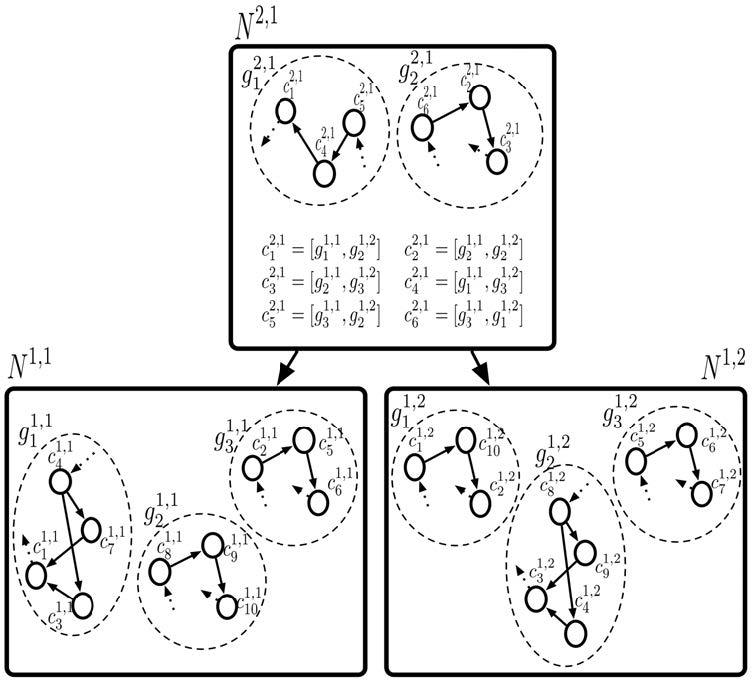
\includegraphics[width=0.7\textwidth]{mpf/hawkins_htm}
				\end{center}
			}
			\only<2>{
				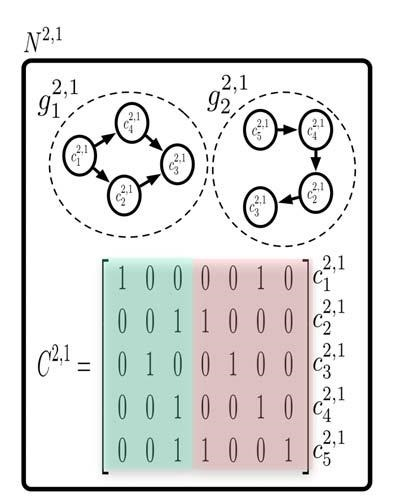
\includegraphics[width=0.4\textwidth]{mpf/hawkins_htm_ex_a}
				\hspace{20mm}
				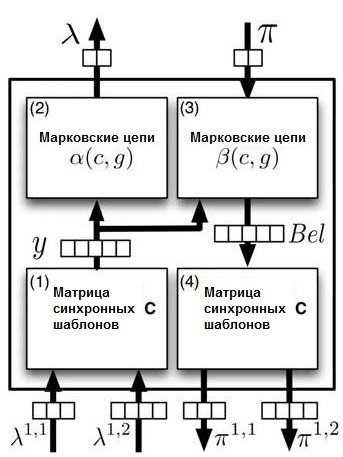
\includegraphics[width=0.4\textwidth]{mpf/hawkins_htm_ex_b}
			}
		\end{overlayarea}
	\end{frame}
	
	\begin{frame}
		\frametitle{Послойная организация}
		
		\begin{columns}
			\begin{column}{0.65\textwidth}
				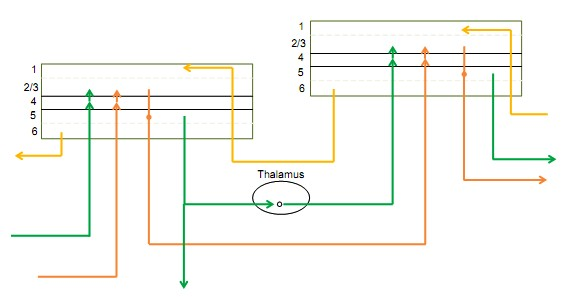
\includegraphics[width=0.9\textwidth]{mpf/regions_connect}
			\end{column}
			\begin{column}{0.35\textwidth}
				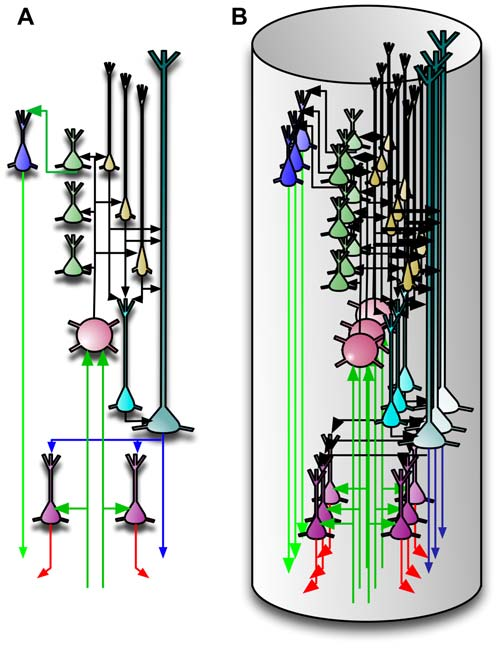
\includegraphics[width=\textwidth]{phisio/column}
			\end{column}
		\end{columns}
	\end{frame}
	
	\begin{frame}
		\frametitle{Образная компонента знака}
		
		При окончании процесса обучения синапсы определяют как вертикальные связи между узлами, так и горизонтальные связи в рамках одного узла.
		\par\bigskip
		Далее будет рассмотрена автоматная модель процесса восприятия, на основе которой будут определены образная компонента знака. 
		\par\bigskip
		Каждому узлу соответствует набор матриц предсказания, которые формируются в результате процесса обучения по алгоритму HTM.
	\end{frame}
			
	\begin{frame}
		\frametitle{Применение для решения интеллектуальных задач}
		
		\begin{itemize}
			\item Моделирование внимания,
			\item образование нового знания (концепта),
			\item планирование поведения,
			\item построение картины мира субъекта на основе текстов,
			\item генерация сообщений на основе картин мира определенного типа (виртуальные ассистенты).
		\end{itemize}
	\end{frame}

	\begin{frame}
		\centering
		\Huge
		Спасибо за внимание!
		\normalsize
		\par\bigskip
		\par\bigskip
		ФИЦ ИУ РАН, лаб. <<Динамические интеллектуальные системы>>, pan@isa.ru
	\end{frame}
														
%	\begin{frame}
%		\frametitle{Цели курса}
%		
%		\begin{columns}
%			\begin{column}{0.5\textwidth}
%				
%			\end{column}
%			\begin{column}{0.5\textwidth}
%				\begin{figure}
%					
\includegraphics[width=\textwidth]{logo}
%				\end{figure}
%			\end{column}
%		\end{columns}
%	\end{frame}
	%	\begin{frame}
	%		\frametitle{Цели курса}
	%		
	%		\begin{itemize}
	%			\item
	%		\end{itemize}
	%	\end{frame}
	
\end{document}
	
	
